%% The first command in your LaTeX source must be the \documentclass command.
%%
%% Options:
%% twocolumn : Two column layout.
%% hf: enable header and footer.
\documentclass[
 twocolumn,
 hf,
]{ceurart}

%%
%% One can fix some overfulls
\sloppy

%%
%% Minted listings support 
%% Need pygment <http://pygments.org/> <http://pypi.python.org/pypi/Pygments>
\usepackage{lmodern}
\usepackage{textcomp}
\usepackage{listings}
\usepackage{minted}

%% auto break lines
\lstset{breaklines=true}

%%
%% end of the preamble, start of the body of the document source.
\begin{document}

%%
%% Rights management information.
%% CC-BY is default license.
\copyrightyear{2022}
\copyrightclause{Copyright for this paper by its authors.
  Use permitted under Creative Commons License Attribution 4.0
  International (CC BY 4.0).}

%%
%% This command is for the conference information
\conference{IJCAI-ECAI 2022, the 31st International Joint Conference on Artificial Intelligence and the 25th European Conference on Artificial Intelligence, July 23--29, 2022
Messe Wien, Vienna, Austria}

%%
%% The "title" command
\title{Understand your clusters: a link between the clustering data and explanatory meta-data}

%%
%% The "author" command and its associated commands are used to define
%% the authors and their affiliations.
\author[1]{Maciej Mozolewski}[
orcid=0000-0003-4227-3894,
email=m.mozolewski@doctoral.uj.edu.pl,
url=https://github.com/mozo64,
]

\author[2]{Samaneh Jamshidi}[
orcid=0000−0001−7055−2706,
email=samaneh.jamshidi@hh.se,
]

\author[1]{Szymon Bobek}[
orcid=0000-0002-6350-8405,
email=szymon.bobek@uj.edu.pl,
]

\author[1]{Grzegorz J. Nalepa}[
orcid=0000-0002-8182-4225,
email=grzegorz.j.nalepa@uj.edu.pl,
]

\address[1]{Jagiellonian Human-Centered Artificial Intelligence Laboratory (JAHCAI) and Institute of Applied Computer Science, Jagiellonian University, Cracow, Poland}
\address[2]{Center for Applied Intelligent Systems Research (CAISR), Halmstad University, Halmstad, Sweden}

%%
%% The abstract is a short summary of the work to be presented in the
%% article.
\begin{abstract}
  In this preliminary work, we present an approach for augmentation of clustering  with Natural Language Explanations.
  In clustering there are 2 main challenges: a) choice of a proper, reasonable number of clusters and b) cluster analysis and profiling.
  There is a plethora of technics for a) but not so much for b), which is in the general a laborious task of explaining obtained clusters.
  %Clustering is in a sense art in that regard that it is an intuitive and iterative process. % This sentence is strange...
  %Therefore, XAI techniques are well suited in this area.
  In this work we propose a method that aids experts in cluster analysis by providing iterative, human-in-the-loop methodology of generating cluster explanations.
  In a convincing example, we show how the process of clustering on a set of "objective" variables could be facilitated with textual metadata.
  In our case images of products from online fashion store are used for clustering.
  Then product descriptions are used for profiling clusters.
\end{abstract}

%%
%% Keywords. The author(s) should pick words that accurately describe
%% the work being presented. Separate the keywords with commas.
\begin{keywords}
  XAI \sep
  clustering \sep
  meta-data \sep
  Natural Language Processing \sep
  explanations \sep
  narratives
\end{keywords}

%%
%% This command processes the author and affiliation and title
%% information and builds the first part of the formatted document.
\maketitle

\section{Introduction}\label{sec:introduction}
%In general what is the prroblem -- in clustering we need to analyse results, XAI can help us in doing that
%- classification as a tool for understanding
Categorization is one of the ways how humans describe the world.
To classify means to notice that some phenomena differ from each other.
And more importantly how they differ.
Finally, one is giving names to those different classes of entities.
Clustering in machine learning in essence is a no different process.

%- the problem is common in fields like: marketing, e-commerce, industries, ???
%- one like to classify "objective" data like images, sensors, etc to uncover hidden structure
%- to many observations to do it manually
Clustering methods are standard in many fields of human prosperity.
In the advent of an ever-increasing amount of data, we use tools to automate the process, as manual clustering is too laborious.
Indeed, there are many statistical, machine learning, and deep learning algorithms.
The difficulty arises to convince end-users that derived clusters make sense.
Will it be clustering sensor data in Industry 4.0 or behaviors of consumers, results need to be actionable.
We believe that this is impossible if we do not explain what the algorithm has learned. % and if it is of any value for humans.
It also follows that the process is iterative.
We continually hypothesize about the significant differences between classes, then test results by looking at classified objects.

%- explanations needs to be done with data comprehensible by humans
%   - data are not equal
%  - images are self-explanatory in e-commerce setting, but not necessarily in other (vide images of medical images, satellites,  etc)
%  - industrial data - rarely
%  - thus "metadata" - link between "objective/hard" data and "soft" - like labels given by humans eg descriptions of products
%  - higher probability of bias
%  - sanity check of metadata
From our expertise in Industry 4.0 and e-commerce, we often see distinctions between 2 types of data.
There are "objective" data and the "subjective" data or "meta-data".
For instance in e-commerce popular approach for recommendations is Collaborative Filtering.
It is based on finding users similar to each other in terms of interactions with products.
Thus, "objective" data are shoppers' behaviors.
Categories, titles, and descriptions of products are "meta-data", which are usually the result of the joint work of many e-store employees.
For rolling steel factories, predictive maintenance models are derived mainly from "objective" sensory data, like temperature, force, etc.
Factory accounting data are "meta-data".
%Six-sigma quality standards lay somewhere in between of "objective-subjective" continuum.

%Our underlying statement is.
%This leads to the conclusion:
The more "objective" data are, the more they are suited for modeling the phenomena, be it physical, business, sociological or psychological in nature.
"Meta-data" are more suited for explaining the model to the user, convincing her or him, and prompt to make decisions and actions based on this knowledge.
They are more prone to error, because of their conventionality and subjectivism, but they speak to humans.
%- one want to have influence on final outcome
%  - as it is exploratory, it is unsupervised
%  - no direct influence -> to adress this ...
%As a closing remark in this section, we want to pinpoint that humans seek agency.
%Clustering algorithms are unsupervised.
%XAI methods are well-fitted for the job of giving control, both in the clustering stage and profiling stage.

In whis work we propose a method that allows for clustering dataset with "objective" data, and explain differences between clusters with meta-data.
We use XAI methods to explain differences between clusters using meta-data which are perfectly understandable by humans, but may not be of enough quality to perform valid clustering.
The selection of most interpretable meta-data is iterative and human-guided.
In our example we show how image-based clustering can be enhanced with textual description of clusters.
We argue that such an approach can lead to better utilisation of meta-data for cluster analysis purposes, which results in better understanding of clusters which is the final goal of every clustering task. % BETTER means nothing, but lets keep it that way.
Furthremore, it allows for checking the consistency between two or more possible instance reporesentations (image and text) which might be crucial in domains that rely on both (e.g.\ e-commerce).



The rest of the paper is organised as follows.
In Section~\ref{sec:sota} we present current research in the area of interactive clsutering and human-guided clsuter analysis.
The description of our method along with use-case studies is given in Section~\ref{sec:clumeta}.
Finally, we conclude our work and show perspectives of its further development is presented in Section~\ref{sec:summary}.

\section{Related works}
\label{sec:sota}
%How this is done in the field
%TODO Parisa

Explainable AI approaches have become particularly important, and although most work is generally focused on supervised learning, some works have been done to explain clusters.
One of the most common methods for understanding clustering methods is visualization. 
By using low-dimensionality embedding and displaying them in two or three dimensions, one can get an overview of the clusters and their data. 
However, these visualizations are not always understandable and explainable. 

The decision tree is one of the inherently interpretable algorithms. 
So one common way to explain models is to use decision trees. 
Nevertheless, the critical point for explaining the decision tree is its depth because decision trees with high depth no longer are interpreted, so we must pay attention to the depth of the tree produced. 
Using a small decision tree to divide a dataset into k clusters provides explainable clusters, but this approach has a trade-off between being explainable and accuracy. 
IMM algorithm approximates k-means and k-median clustering by a threshold tree with k leaves.
While ExKMC uses a threshold tree to provide an explainable k-mean clustering in which the number of tree leaves is more than the number of clusters.

Besides visualization or providing some conditions on features, using text data is reasonable to explain to users. 
~\cite{hendricks2016generating} uses the captions of the images along with images to create a more discriminative classification. 
In addition, they use this meta-data to provide language explanation and generate a text description for each class.

Another approach is given in~\cite{knac2021arxiv}, where authors present a toolkit for conformance checking between expert knowledge with automatic clastering.
The differences in expert-based clustering and automated clustering is justified with XAI methods and the process is iterative.
However, the explanations are not human-guided, and the expert has no impact on the way they are generated.
In particular it is not possible to provide additional meta-data for explanations, nor modify the set of conccepts that are used for explanations.


\section{Cluster analysis with meta-data}
\label{sec:clumeta}
In this section, we will show how our method could be applied to real case scenarios.
We choose an example from the e-commerce field because the authors have experience working in this industry.
Specifically, we work with online stores to provide them, among others, with recommendations of products to their end-users (clients).

In real-life scenarios, data about products are stored in product catalogs in shop databases, and most often exchanged with so-called product feeds (XML documents).
We used a public dataset from Kaggle\footnote{See: \url{https://www.kaggle.com/datasets/paramaggarwal/fashion-product-images-small}}.
This dataset in terms of content resembles a product feed for an online store of a medium size product catalog.
It consisted of 44000 products with category labels, titles, and images.

%Our workflow was based on this Kaggle notebook: https://www.kaggle.com/code/shubhijoshi/similar-image-finder-using-k-means/notebook, and we adapted it to our needs.
As been said before, we treat images as "objective" data.
We used embeddings of images obtained via MobileNetV2~\cite{sandler2019mobilenetv2}.
The fully-connected layer at the top of the network was disregarded because we were not interested in the classification done by the model.
The output of the final layer of the model was of length 20480.
We used Singular Value Decomposition (SVD) with normalization to reduce the dimensionality of embeddings, leaving at least 90 percent of the variance.

%Description of the algorithms, results on synmthetic data
% We are aiming for the most general case of user exploratory analysis.
% We assume that user performs exploratory analysis. % and not necessarily has exhaustive knowlaedge.
% Our work is WIP.
%- Usually clustering consists of 2 steps:
%  - choice of number of clusters
%  - profiling
%  - repetitive process
%- we propose to explain clusters derived from 1 modality ("hard data") with textual modality (usual form of metadata)
%- for choice of clusters: TSNE and silhouette score
In this section, we will present tools dedicated to data scientists who would like to perform clustering.
We propose a 2-step clustering loop, which consists of k-means clustering and textual explanations of clusters.
Data preparation also could be performed more than once, if needed.
For the sake of simplicity, we call it "step 0" in this work.

\subsection{Data preparation}\label{subsec:data-preparation}
The method requires 2 types of data: "objective" and "meta-data" as defined in the previous section.
In "step 0" method provides users with helper functions to prepare both types of data.
For "objective" data there is a function that performs a reduction of dimensionality via SVD followed by normalization.
It works on any numerical data, which could be as well as one-hot variables and continuous real values (floats).
User sets percent of explained variance left after SVD reduction.
The optimal count of new dimensions could be determined automatically by our algorithm.
This is done by probing different dimension counts with scipy.optimize package, so the user does not need to do this manually.
As for "meta-data" which are textual, there are wrappers built on top of SpaCy and NLTK libraries.
Users can contact text columns, lemmatize, remove stopwords and perform Tf-Idf vectorization.
For numerical "meta-data", we found a way to incorporate them into textual explanations.
For instance, the year could be recoded as the label "year2022", which will be easily interpreted along the pipeline.
Other numerical variables could be recoded to low/medium/high bins, based on quartiles.
Finally, the user constructs the "Pipeline" object and initializes it with 2 datasets: "objective" and "meta-data".
%User can also define functions for creating observation labeles, which could be passed to constructor.

\subsection{Assitance in clustering}\label{subsec:assitance-in-clustering}
The first step corresponds to running the unsupervised algorithm.
Typically, the person who performs the analysis starts with the dilemma of choice of the number of clusters.
It can be resolved with her/his background knowledge, intuition, practicality prerequisites, or just a trial and error approach. %  in terms of comprehension of output and
To give our users a hint in this regard, we use the T-SNE 2-dimensional projection of the data.
At the moment, this is a solely visual clue.
It is depicted on Figure~\ref{fig:tsne}.
\begin{figure}[h!]
  \centering
  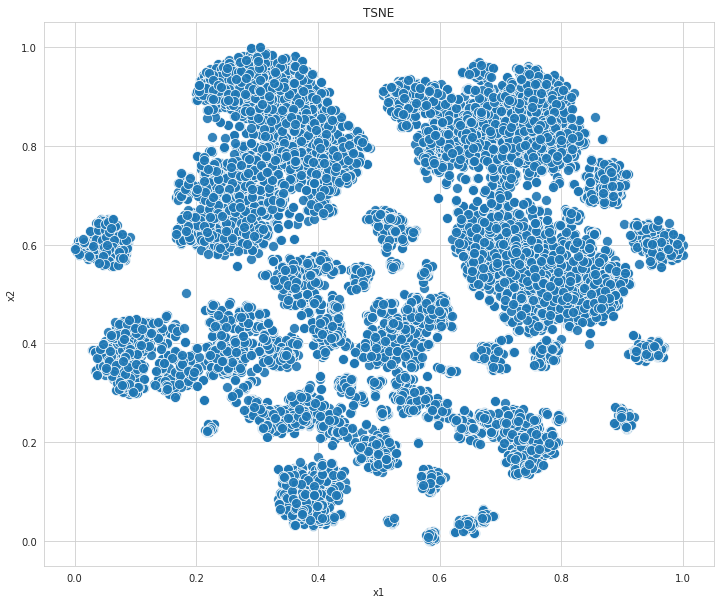
\includegraphics[width=\linewidth]{example1-clustering-products-fashion-tex/output_57_1}
  \caption{Preliminary visualisation of "objective" data in 2-D projection}
  \label{fig:tsne}
\end{figure}
If data have an underlying structure, points representing observations will cluster, which would be observed on the chart.
As T-SNE on massive data could be resource intensive, the default is to run this process on random subsample and cache results.
Additionally, users can apply textual labels to the T-SNE chart, plotted on a subsample of data, to avoid cluttering the chart. % , prepared in {Data preparation}
Labels could represent the most important pieces of "meta-data", like the label, observation id, and summary of description.
The next clue is derived from the silhouette score on a plot in the Figure~\ref{fig:silhouette}.
\begin{figure}[h!]
  \centering
  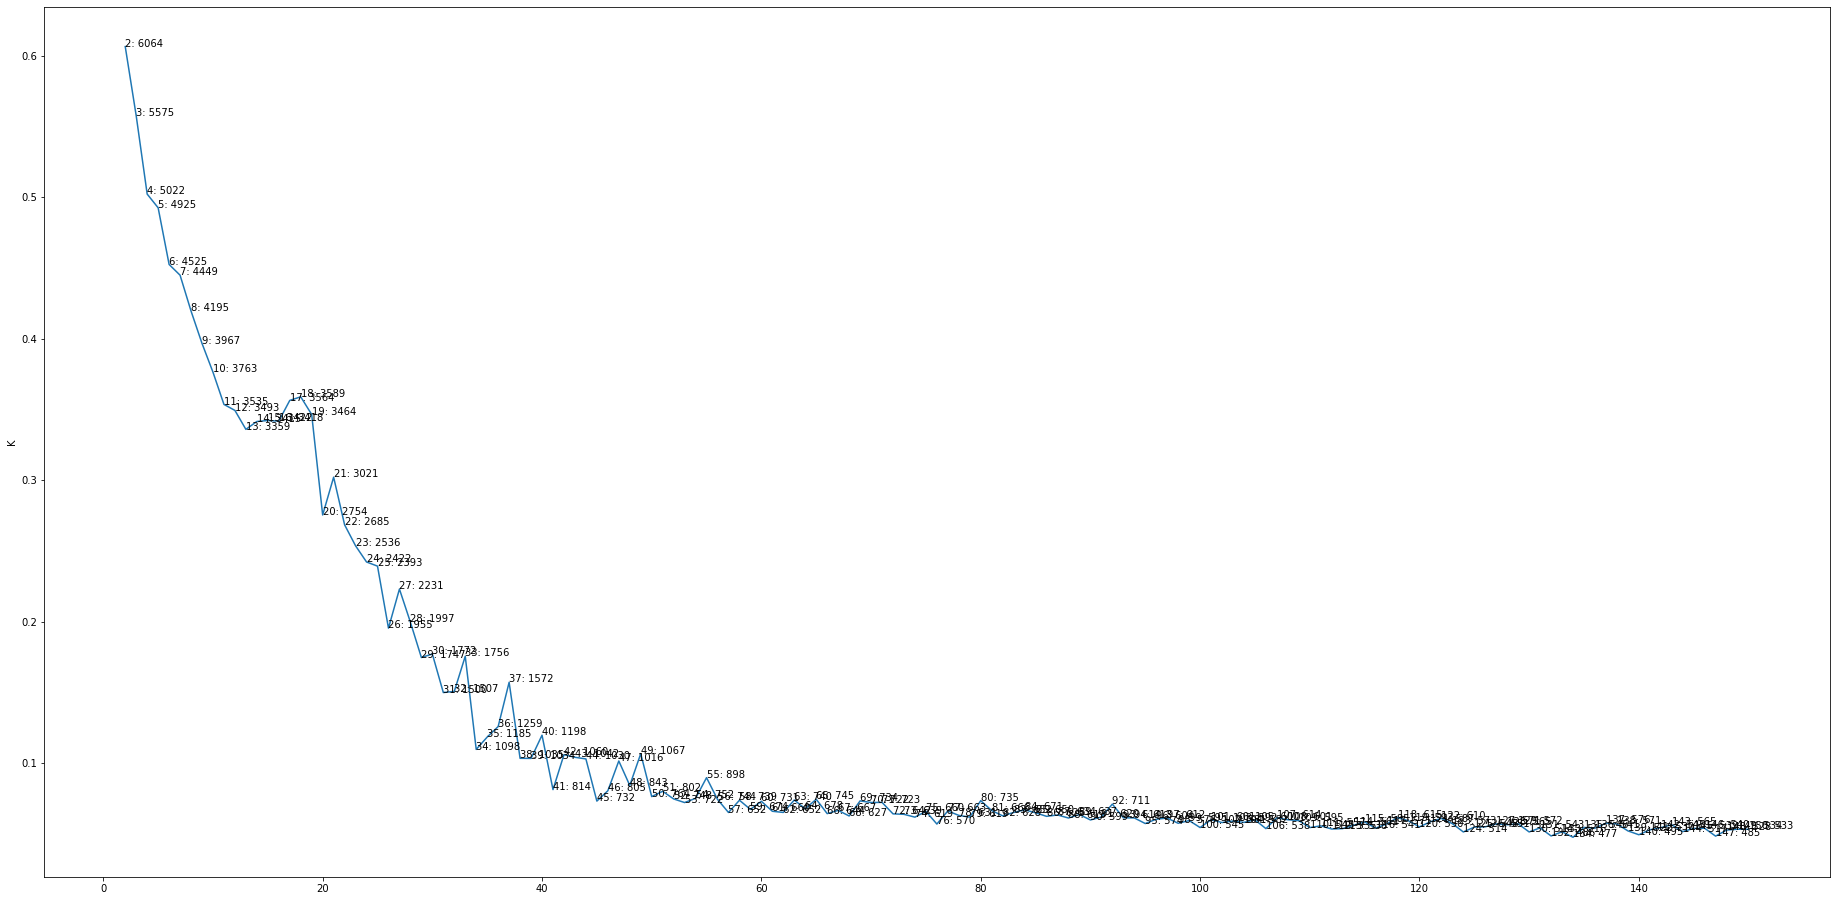
\includegraphics[width=\linewidth]{example1-clustering-products-fashion-tex/output_58_0}
  \caption{Silhouette score with cluster counts and values}
  \label{fig:silhouette}
\end{figure}
The range of the number of clusters to be tested is provided in accordance with the previous clue.
To speed-up computations, this plot could be obtained on a random subset, and results are cached for further reference.
For now, the user interprets the plot on her/his own.
Finally, clustering with k-means is performed on all observations.
Visualization with T-SNE is presented, this time with clusters colored different colors, which is depicted on Figure~\ref{fig:kmeans}.
\begin{figure}[h!]
  \centering
  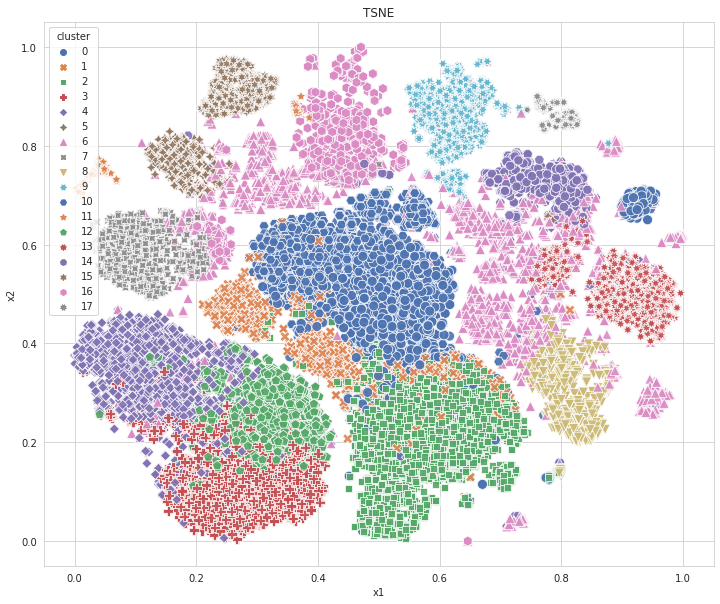
\includegraphics[width=\linewidth]{example1-clustering-products-fashion-tex/output_59_0}
  \caption{Preliminary visualisation of "objective" data in 2-D projection}
  \label{fig:kmeans}
\end{figure}

\subsection{Interactive explanations}\label{subsec:interactive-explanations}
%- then textual explanations follows straight away
The second step is to explain clusters, so the person who performs data analysis can assess the result.
We would like to give users agency in refining explanations.
Thus, we provide her or him with the possibility to influence explanations by extending stopwords with his own terms.
On the other hand, we initialize the whitelist with keywords like "year2022", defined in "step 0".
Then we use the Tf-Idf vectorizer, taking into account the aforementioned lists.
Vectors are used for training decision tree classifiers.
The size of the list of additional terms is under the control of a user.
She or he can change it and interactively observe the changes in a Figure~\ref{fig:decision_tree}.
Moreover, there are presented example observations on Figure~\ref{fig:example_products}, word clouds describing clusters on Figure~\ref{fig:wordcloud} and LIME explanation for one instance of meta-data Figure~\ref{fig:lime}.
\begin{figure}[h!]
  \centering
  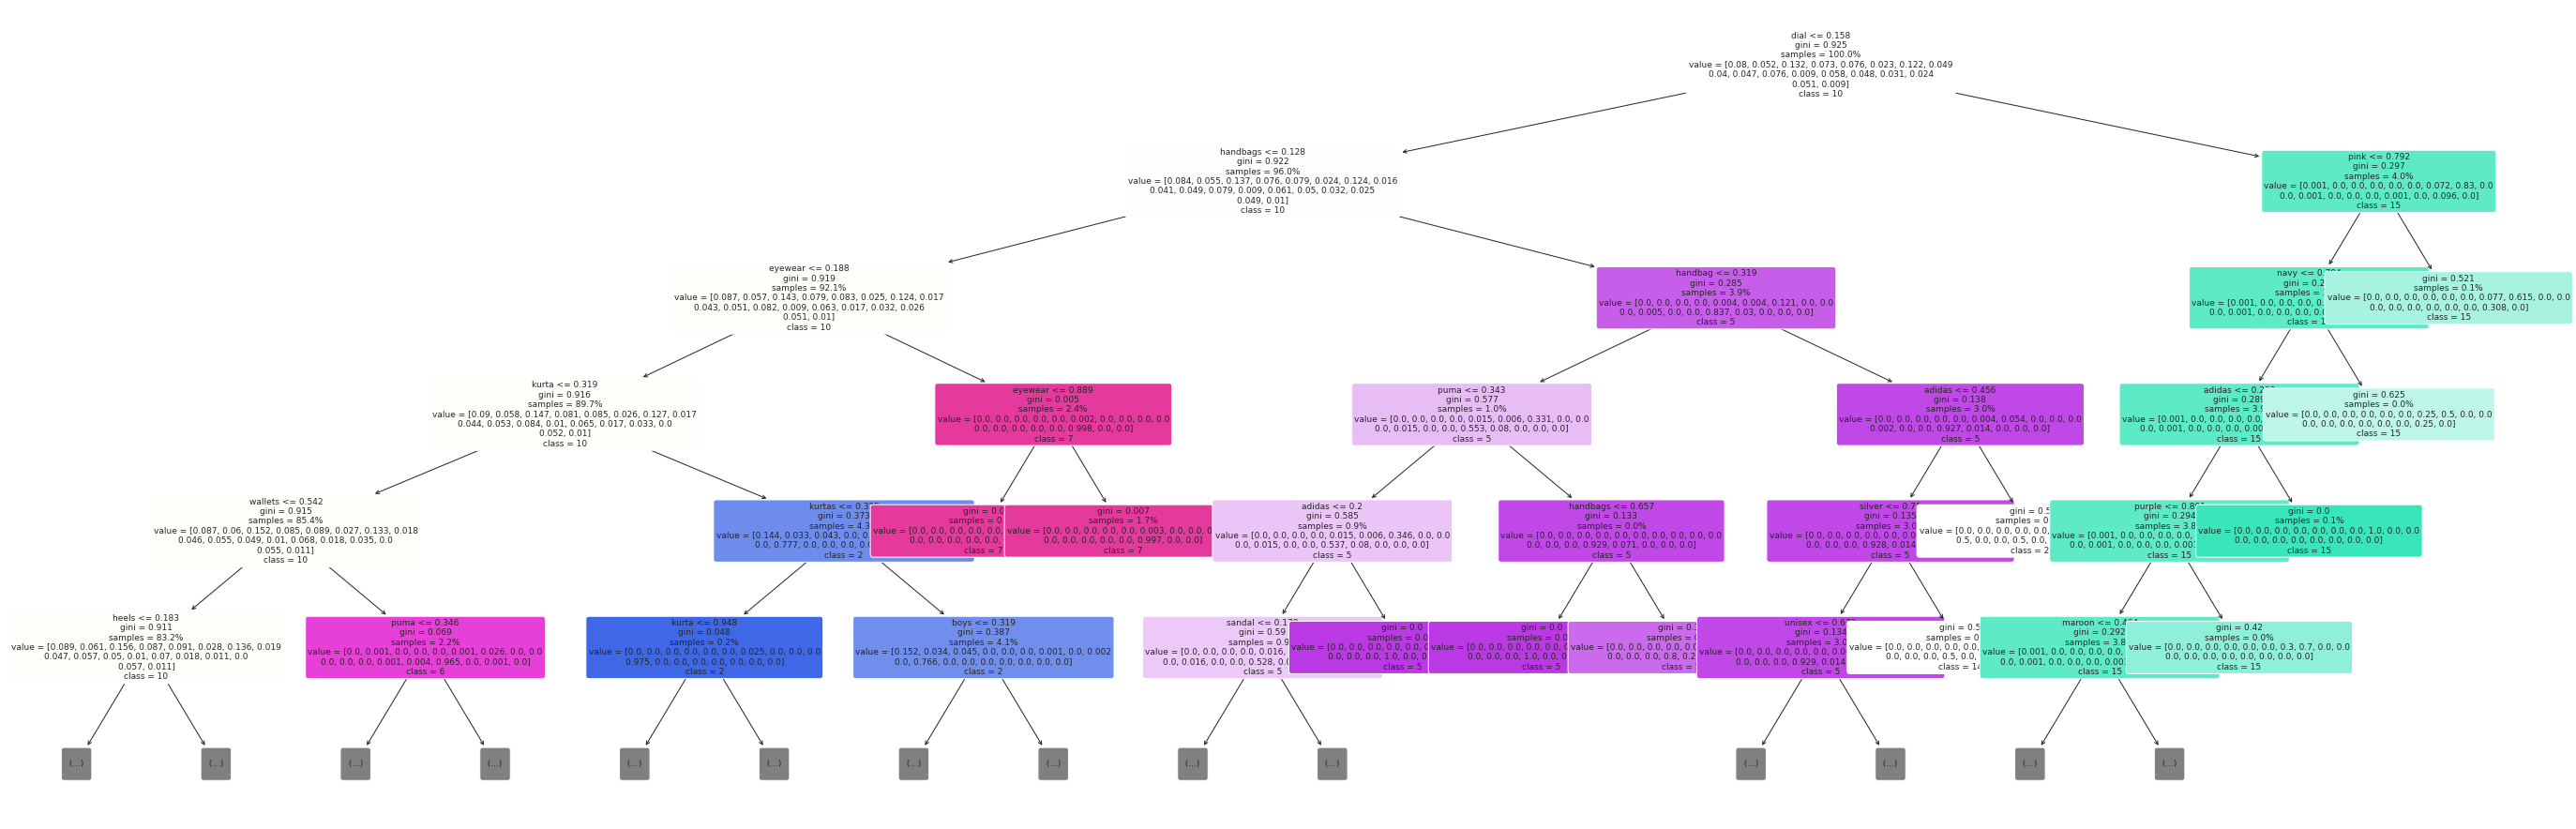
\includegraphics[width=\linewidth]{example1-clustering-products-fashion-tex/output_61_2}
  \caption{Decision tree classifier which explains how clusters differ in terms of metadata}
  \label{fig:decision_tree}
\end{figure}
The last stage is a plot of the word cloud of each cluster, using the same Tf-Idf vectorizer.
Plots are accompanied by examples of observations if data scientists should define visualization function and pass into Pipeline class API\@.
Moreover, there is random observation with the LIME explainer for a given class.
\begin{figure}[h!]
  \centering
  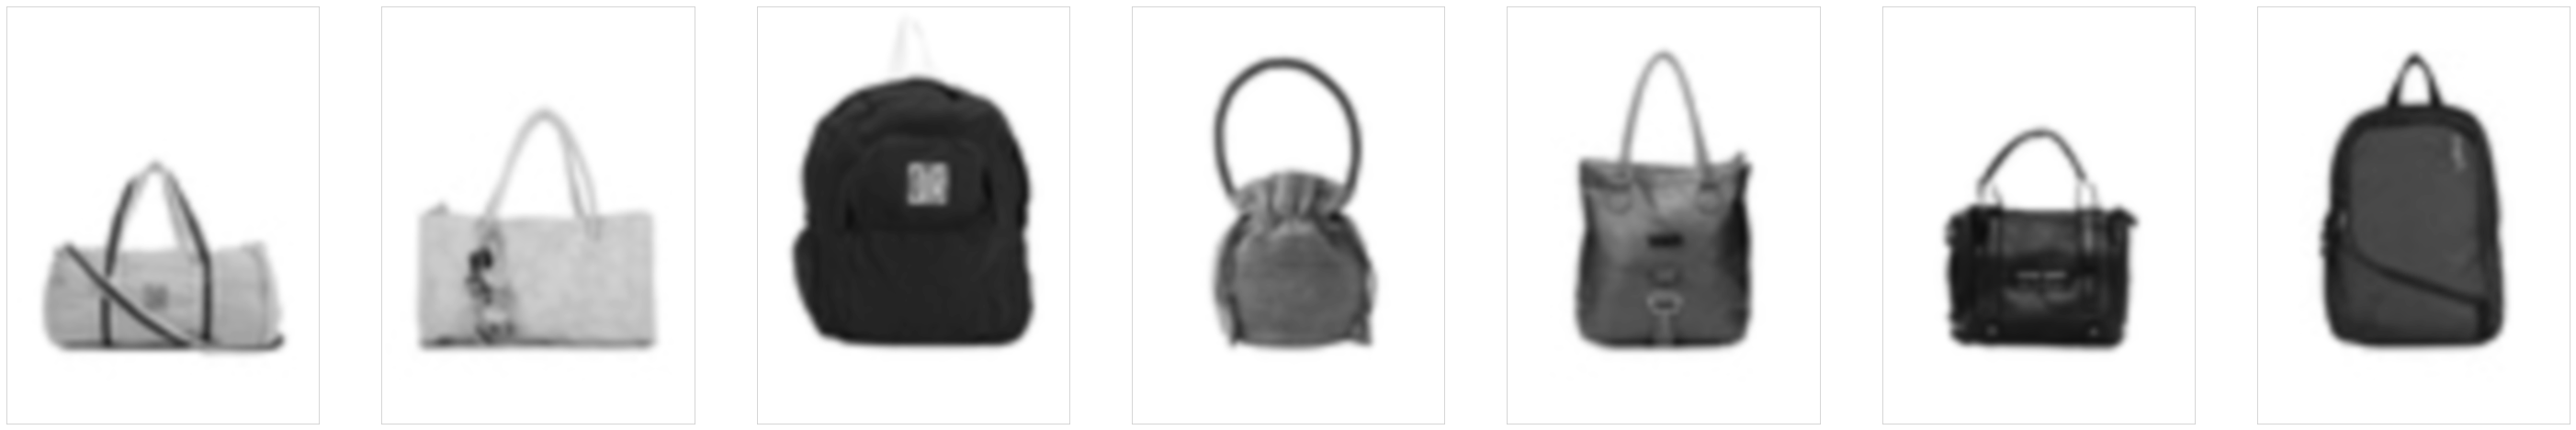
\includegraphics[width=\linewidth]{example1-clustering-products-fashion-tex/output_62_22}
  \caption{Example products}
  \label{fig:example_products}
\end{figure}
\begin{figure}[h!]
  \centering
  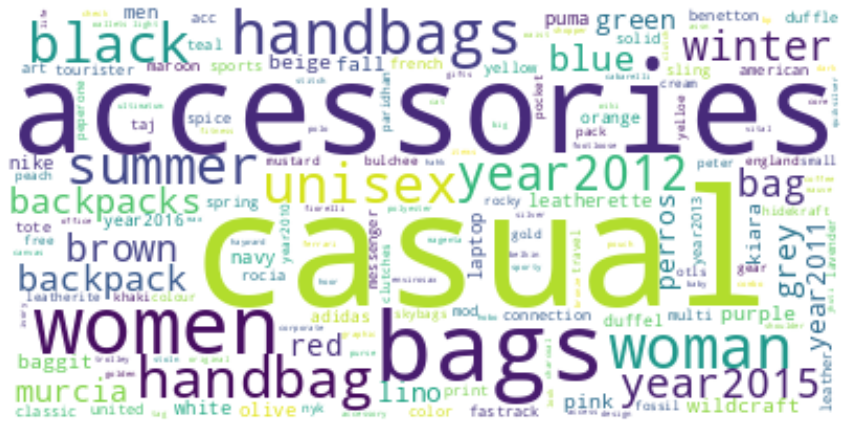
\includegraphics[width=\linewidth]{example1-clustering-products-fashion-tex/output_62_23}
  \caption{Word cloud for a given category}
  \label{fig:wordcloud}
\end{figure}
\begin{figure}[h!]
  \centering
  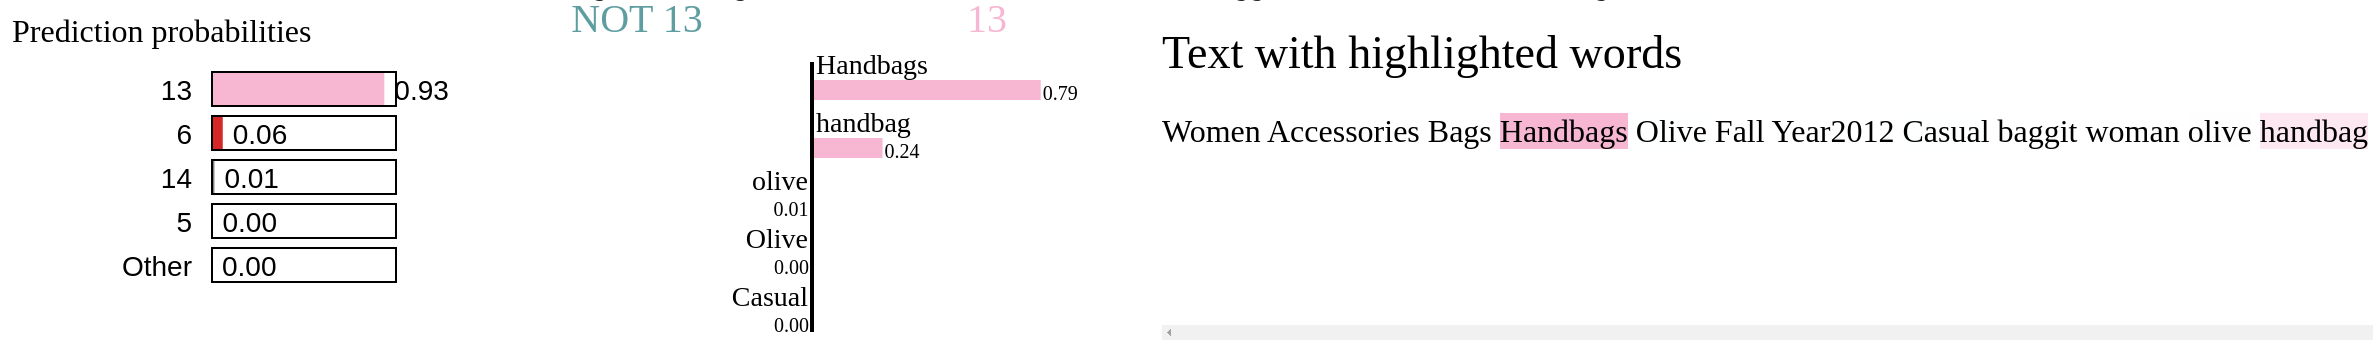
\includegraphics[width=\linewidth]{example1-clustering-products-fashion-tex/LIME_13_handbags-Selection_265}
  \caption{LIME explanation for observation in category "handbags"}
  \label{fig:lime}
\end{figure}

%\section{Real case scenario}
%So far we tested our approach on 2 cases.
%We provide user with Pipeline class, which works in Python environment, like Jupyter notebooks.
%%, which API consist of methods:
%%About the paper citation clustering  and what are plans for extending that part.
%
%Textual data was processed as follows:


\section{Summary}
\label{sec:summary}
%We believe that the XAI methods are most useful when they support human work.
%The main purpose of this paper is to show that XAI can be put into practice when it is based on 2 foundations.
%The first is the need for a dialogue between the machine learning system and its user, taking into account the needs and predispositions of the latter.
In this work we presented the method that allows for explaining clusters with concepts that could be more human-readable that data which was used as sn input to clustering algorithm.
We based our method on the observation that different types of data are suitable in different degrees to clustering and explaining tasks.
We demonstrated the feasibility of our approach on the e-commerce example, where images were treated as input for clustering and textial descriptions of images as basis for cluster descriptions.

%Our approach is obviously not new, but it is worth emphasizing if one wants to create useful solutions for machine learning practitioners.
%We have developed a method that relates to the cluster analysis method, as this technique is widely used with a broad spectrum of applications in science, industry, business, and marketing.
%Furthermore, it is easy to show that it is actually a technical extension of the natural process of describing reality.
%It is also clearly an iterative process, so it is a form of a dialogue between humans and algorithms, and understanding is even more important than, for example, in regression techniques.

%- deep learning - how to use meta-data in DL ?
%- NLG for explanations
In future work we would like to improve our method with several extensions.
We will focus on automatically proposing number of clusters based both on embedding features with technics similar to T-SNE and metrics like silhouette score.
We want to test other techniques clustering than k-means.
For instance hierarchical clustering could more suited in e-commerce, where taxonomies of products are multilayer.
Word clouds could be replaced with topic analysis with Latent Dirichlet Allocation or techniques derived from Natural Language Generation.
Another interesting direction is to construct explanations with other modalities, like visual, by something more sophisticated than presenting example images.
It could be done for instance with image captioning.


%We are already working on applications of the tool
%- e-commerce: customer segmentation, SEO
%-

%:)

\begin{acknowledgments}
The work of Szymon Bobek has been additionally supported by a HuLCKA grant from the Priority Research Area (Digiworld) under the Strategic Programme Excellence Initiative at the Jagiellonian University (U1U/P06/NO/02.16).

The work of Samaneh Jamshidi was supported by CHIST-ERA grant CHIST-ERA-19-XAI-012 funded by Swedish Research Council.
\end{acknowledgments}

%%
%% Define the bibliography file to be used
%\nocite{*}
\bibliography{sample-ceur}
%\bibliographystyle{plain}

% TODO Szymon




\end{document}

%%
%% End of file
